\subsection{Structured-Control-Flow Construct}

Translating from stack-based IR to register-based IR is not trivial, especially when non-linear control flow structures appeared. This problem appeared in many runtime system implementations, such as Numba \cite{numba}, a just-in-time (JIT) compiler for Python. Usually, one needs some algorithm to recover the control flow structure from annoying jump instructions. Luckily, in WebAssembly, we can translate the stack-based bytecode into register-based basic blocks in linear time, thanks to the structured-control-flow constructs and their validation rules defined in WebAssembly. In this section, we will cover the translation pattern used for WebAssembly's structured-control-flow constructs, namely \texttt{block}, \texttt{if} and \texttt{loop}.

\begin{figure}
  \centering
  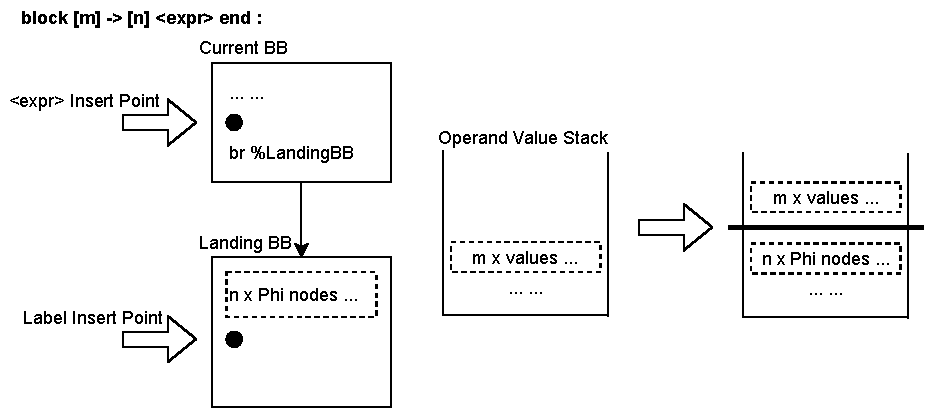
\includegraphics[width=\textwidth]{Images/4.MIR/translate-block.pdf}
  \caption{WebAssembly \texttt{block} translation pattern}
  \label{fig:translate-block}
\end{figure}

\begin{figure}
  \centering
  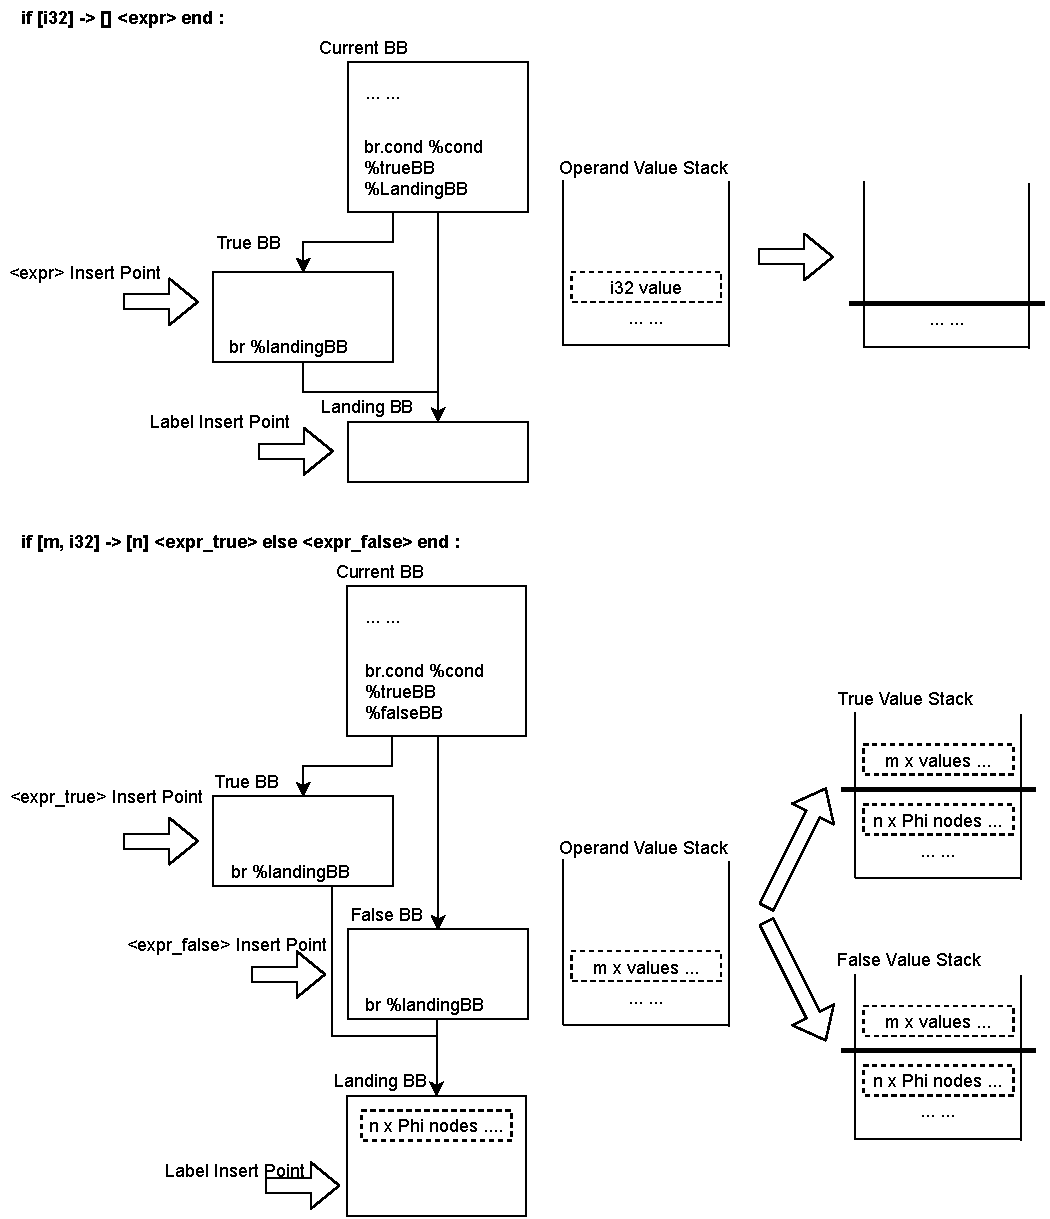
\includegraphics[width=\textwidth]{Images/4.MIR/translate-if.pdf}
  \caption{WebAssembly \texttt{if} translation pattern}
  \label{fig:translate-if}
\end{figure}

\paragraph{Block} In the background chapter, we provide a general illustration of the three structured-control-flow constructs.  As a quick recap, \texttt{block} is the simplest form of a structured-control-flow construct. It implicitly introduces a label at the end of its enclosing instructions. A branching instruction referring to this label will redirect the control flow to the end of the block. Figure~\ref{fig:translate-block} illustrates the translation pattern for WebAssembly \texttt{block} in SableWasm MIR.  We will first clarify some of the terminologies we used in the figure, and we will use the same terms later in the \texttt{loop} and \texttt{if} pattern discussion. \emph{Expr Insert Point} refer to the starting position for the generated instructions when we recursively translate the instructions within the enclosing expression of the \texttt{block} instruction. Furthermore, \emph{Label Insert Point} refer to the position for generated instruction when we finish the recursive translation and resume to the parent expression of the \texttt{block} instruction. A \emph{label stack entry} is a tuple consisting of a pointer to the landing BB, a list of Phi nodes expecting merge values, and a pointer to the \emph{label insert point}. The translation pattern for \texttt{block} is pretty simple; we continue on the current BB and prepare the landing BB for the block instruction as the branch instructions within the nested expression may refer to the label. Additionally, to fully support multi-value extension in WebAssembly, we need also to prepare the Phi nodes in the landing BB. SableWasm generates the Phi nodes from the type of the \texttt{block} instruction. WebAssembly validation ensures that the nested expression can access exactly $m$ values from the stack and put $n$ values onto the stack. Finally, we will append an unconditional branching to the landing BB because in WebAssembly, if the control flow reaches the bottom of the \texttt{block} expressions, it will implicitly fall through. For operand stack, we will first pop $m$ values from the stack as \texttt{block} instruction's type suggests and push the Phi nodes as the result values. Now we need to set up the operand stack for our nested expression. Again, due to the WebAssembly validation rule, we need to insert a boundary before continuing. Figures~\ref{fig:translate-block} represents this with the bold line in the result operand value stack. We create a new operand value-stack during recursive translation instead of using some magic stack elements in practice.  Because the nested can access $m$ values from the parent stack, finally, we push the $m$ values onto the new stack.


\paragraph{If} The next control-flow structure defined WebAssembly in \texttt{if}. \texttt{if} is very similar to a \emph{if} statement that appears in many other programming languages. Figure~\ref{fig:translate-if} illustrates the translation patterns that used in SableWasm.